\documentclass[11pt]{article}
\usepackage[english]{babel}
\usepackage[utf8]{inputenc}
\usepackage{amsmath}
\usepackage{amssymb}
\usepackage{amsthm}
\usepackage{color}
\usepackage[margin=1in,nohead]{geometry}
\usepackage[mathscr]{euscript}
\usepackage{enumitem}
\usepackage{url}
\usepackage{hyperref}
\usepackage{graphicx}
\usepackage{subcaption}
\usepackage{listings}

\newcommand{\mc}{\mathcal}
\newcommand{\mbf}{\mathbf}
\newcommand{\mb}{\mathbb}
\newcommand{\msc}{\mathscr}
\newcommand{\goesto}{\rightarrow}
\newcommand{\note}{{\bf Note: }}
\newcommand{\vspan}{\text{span}}

\newcommand{\R}{\mb{R}}
\newcommand{\nat}{\mb{N}}

\newcommand{\A}{\mathbf{A}}
\newcommand{\B}{\mathbf{B}}
\newcommand{\C}{\mathbf{C}}
\newcommand{\x}{\mathbf{x}}
\newcommand{\y}{\mathbf{y}}
\newcommand{\z}{\mathbf{z}}
\renewcommand{\b}{\mathbf{b}}
\renewcommand{\u}{\mathbf{u}}
\renewcommand{\v}{\mathbf{v}}
\newcommand{\ones}{\mathbf{1}}
\newcommand{\zero}{\mathbf{0}}

\newcommand{\Eqn}[1]{\begin{align*} #1 \end{align*}}
\newcommand{\bbm}{\begin{bmatrix}}
\newcommand{\ebm}{\end{bmatrix}}
\newcommand{\bpm}{\begin{pmatrix}}
\newcommand{\epm}{\end{pmatrix}}

\newcommand{\Sol}{\par {\bf Solution:}}
\newcommand{\sample}[1]{#1_1 , \dots , #1_n}

\setlength{\parskip}{6pt}
\setlength{\parindent}{0pt}
\allowdisplaybreaks[4]
\lstset{
  basicstyle=\ttfamily,
  columns=fullflexible,
  frame=single,
  breaklines=true,
  postbreak=\mbox{\textcolor{red}{$\hookrightarrow$}\space},
}


\begin{document}

\begin{center}
\Large{
\textbf{CSE 691, Spring 2023, Homework 2} \\
Due: Wednesday, Feb 08, 2023. \\
Shu Wan (1226038322)
}
\end{center}
%\bigskip

\section*{A Stochastic Investment Problem}

This exercise deals with a computational comparison of the optimal policy, a heuristic policy, and on-line approximation in value space using the heuristic policy, in the context of the following problem. An investor wants to sell a given amount of stock at any one of $N$ time periods. The initial price of the stock is an integer $x_0$. The price $x_k$, if it is positive and it is less than a given positive integer value $\bar x$, it evolves according to
\begin{equation}\label{eq:1}
x_{k+1} = \begin{cases}
x_{k} + 1 & \text{with probability } p^+, \\
x_{k} & \text{with probability } 1 - p^+ - p^-, \\
x_{k} - 1 & \text{with probability } p^-,
\end{cases}
\end{equation}
where $p^+$ and $p^-$ have known values with
\[
0 < p^- < p^+, \quad p^+ + p+- < 1.
\]

If $x_k = 0$, then $x_k+1$ moves to 1 with probability $p^+$, and stays unchanged at 0 with probability $1 -p^+$. If $x_k = \bar x$, then $x_{k+1}$ moves to $\bar x - 1$ with probability
$p^-$, and stays unchanged at $\bar x$ with probability $1 -p^-$. 

At each period $k = 0, \dots, N - 1$ for which the stock has not yet been sold, the investor (with knowledge of the current price $x_k$), can either sell the stock
at the current price $x_k$ or postpone the sale for a future period. If the stock has not been sold at any of the periods $k = 0, . . . ,N - 1$, it must be sold at period
$N$ at price $x_N$. The investor wants to maximize the expected value of the sale.
For the following computations, use reasonable values of your choice for $N$, $p^+$,
$p^-$, $\bar x$, and $x_0$ (you should choose $x_0$ between 0 and $\bar x$). You are encouraged to experiment with different sets of values. A set of values that you may try first is
\begin{equation}\label{eq:2}
    N = 14, ~x_0 = 3, ~\bar x = 7, ~p^+ = p^- = 0.25.
\end{equation}

\begin{enumerate}[label=(\alph*)]
    \item Formulate the problem as a finite horizon DP problem by identifying the state, control, and disturbance spaces, the system equation, the cost function, and the probability distribution of the disturbance. Write the corresponding exact DP algorithm, and use it to compute the optimal policy and the optimal cost as a function of $x_0$.
    \item Suppose the investor adopts a heuristic, referred to as base heuristic, whereby he/she sells the stock if its price is greater or equal to $\beta x_0$, where $\beta$ is some number with $\beta > 1$. Write an exact DP algorithm to compute the expected value of the sale under this heuristic.
    \item Apply approximation in value space with one-step lookahead minimization and with function approximation that is based on the heuristic of part (b). In particular, use $ \tilde J_N(x_N) = x_N$, and for $k = 1, \dots ,N -1$, use $\tilde J_k(x_k)$ that is equal to the expected value of the sale when starting at $x_k$ and using the heuristic that sells the stock when its price exceeds $\beta x_k$. Use exact DP as well as Monte Carlo simulation to compute/approximate on-line the needed values $\tilde J_k(x_k)$. Compare the expected values of sale price computed with the optimal, heuristic, and approximation in value space methods.
    \item Repeat part(c) but with two-step instead of one-step lookahead minimization.
\end{enumerate}

\Sol

\begin{enumerate}[label=(\alph*)]
    \item
    We formulate the investment problem as a stochastic DP problem over $N, k \in \{0, \dots, N\}$ stages with the stock's price as the state $x_k$, selling decision as the control $u_k$, and the price change probability $\boldsymbol p \in \{\mathcal{P}:(p^+, 1 - p^+ - p^-, p^-)\}$ as the random disturbance.
    The system equation $x_{k+1} = f_k(x_k, u_k, p_k)$ is given in Eq. (\ref{eq:1}).
    
    We can unify all cases with the following formulation,
   \begin{equation}\label{eq:3}
    x_{k+1} = f_k^*(x_k, u_k, p_k) = \begin{cases}
    \min(x_{k} + 1, \bar x) & \text{with probability } p^+, \\
    x_{k} & \text{with probability } 1 - p^+ - p^-, \\
    \max(x_{k} - 1, 0) & \text{with probability } p^-.
    \end{cases}
    \end{equation}
    This is also equivalent to define a clamp function $x_{k+1}^* = c(x_{k+1}) = \max(\min(x_{k+1}, \bar x), 0)$ with corresponding probability. The clamp function constrain the price within the boundary. In later parts, we'll see how this formulation simplifies the algorithm.
    
    Unlike other DP problems, we use \emph{reward} instead of \emph{cost} as the optimization goal as it's more straightforward in an investment problem. The reward is defined as the stock price $g_k(x_k, u_k, p_k) = x_k$ if sold $u_k = 1$ at $k$. Here, the reward is defined without subtracting the initial price $x_0$ because subtracting a fixed number does not impact the decision. It's also worth noting that the reward is not cumulative; selling stock only happens once.
    
    The optimal reward-to-go function $J_k^*(x_k)$ is the optimal solution of the sub-problems start at $k$.
    When $k = N$, we have
    \[
    J_N^*(x_N) = x_N,
    \]
    and for $k = 0, \dots, N-1$, if $x_k = \bar x$, then
    \[
    J_k^*(x_k) = J_k^*(\bar x) = \bar x,
    \]
    if $x_k = 0$, then
    \[
    J_k^*(x_k) = J_k^*(0) = p^+J^*_{k+1}(1) + (1-p^+)J^*_{k+1}(0),
    \]
    and if $0 < x_k < \bar x$, then
    \begin{equation}\label{eq:4}
       J_k^*(x_k) = \max \{x_k, E_{p_k}[J^*_{k+1}(f_k(x_k, u_k, p_k))]\},
    \end{equation}
    where
    \[
    E_{p_k}[J^*_{k+1}(f_k(x_k, u_k, p_k))] = p^+J^*_{k+1}(x_k + 1) + p^-J^*_{k+1}(x_k - 1) + (1-p^+-p^-)J^*_{k+1}(x_k).
    \]
    In fact, if we adopt the formulation of Eq. (\ref{eq:3}), we can unify all cases in one equation: 
    \begin{equation}\label{eq:5}
       J_k^*(x_k) = \max \{x_k, E_{\boldsymbol p}[J^*_{k+1}(f^*_k(x_k, u_k, \boldsymbol p))]\},
    \end{equation}
    The optimal policy $u^*_k$ at time $k$ is given by
    \[
    u^*_k = \begin{cases}
        1 ~(\text{Sell})& \text{if } x_k = J_k^*(x_k),\\
        0 ~(\text{Keep}) & \text{otherwise}.
    \end{cases}
    \]
    That is, we only sell stock when $x_k$ attains the maximum reward at time $k$. When $k < N$, if $x_k = 0$, then it's optimal not to sell and it's optimal to sell when $x_k = \bar x$.

    The exact DP algorithm needs to compute $J_k^*$ for all $k$, beginning with $N$ and work backwards. For each stage $k$, we calculate expected reward $E_{\boldsymbol p}[J^*_{k+1}(f_k(x_k, u_k, p_k))]$. After all rewards are computed, we can generate the optimal policy at the time $k$ by traversing forward.
    
    We use the given parameters to showcase the exact DP algorithm.
    \begin{figure}[h]
    \begin{subfigure}{0.5\textwidth}
    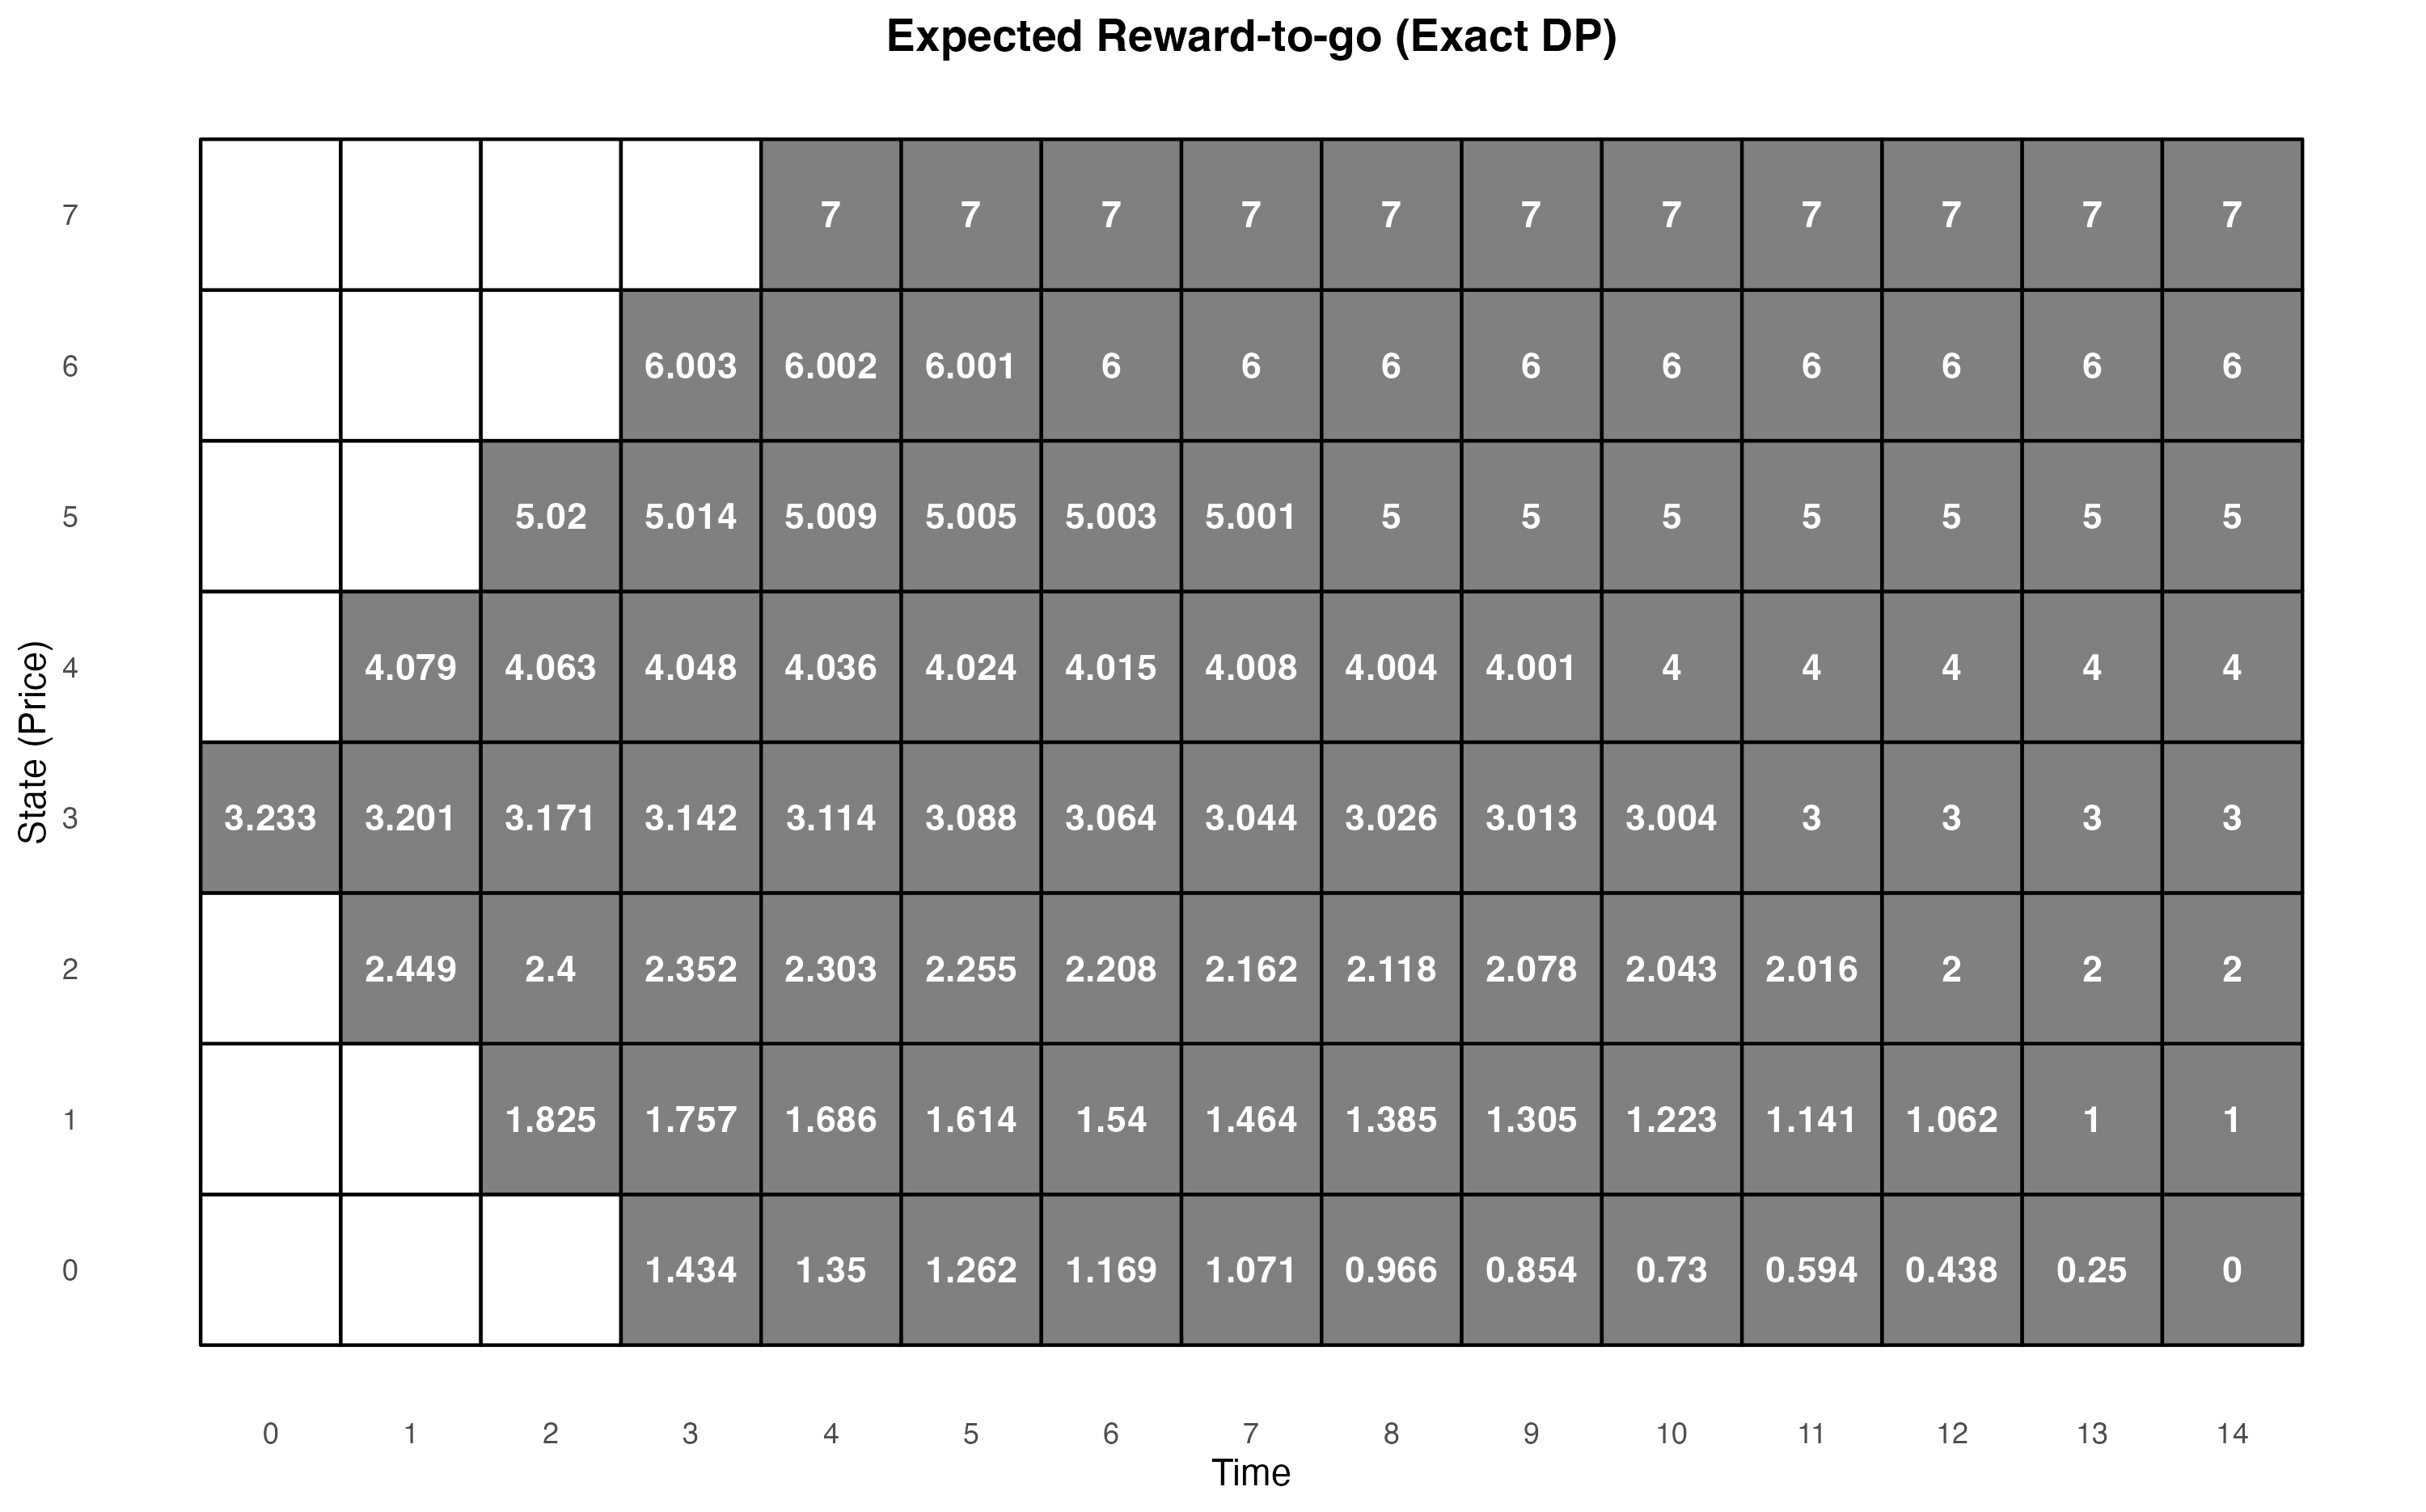
\includegraphics[width=0.9\linewidth, height=6cm]{media/hw2/parta1.png} 
    \label{fig:parta1}
    \end{subfigure}
    \begin{subfigure}{0.5\textwidth}
    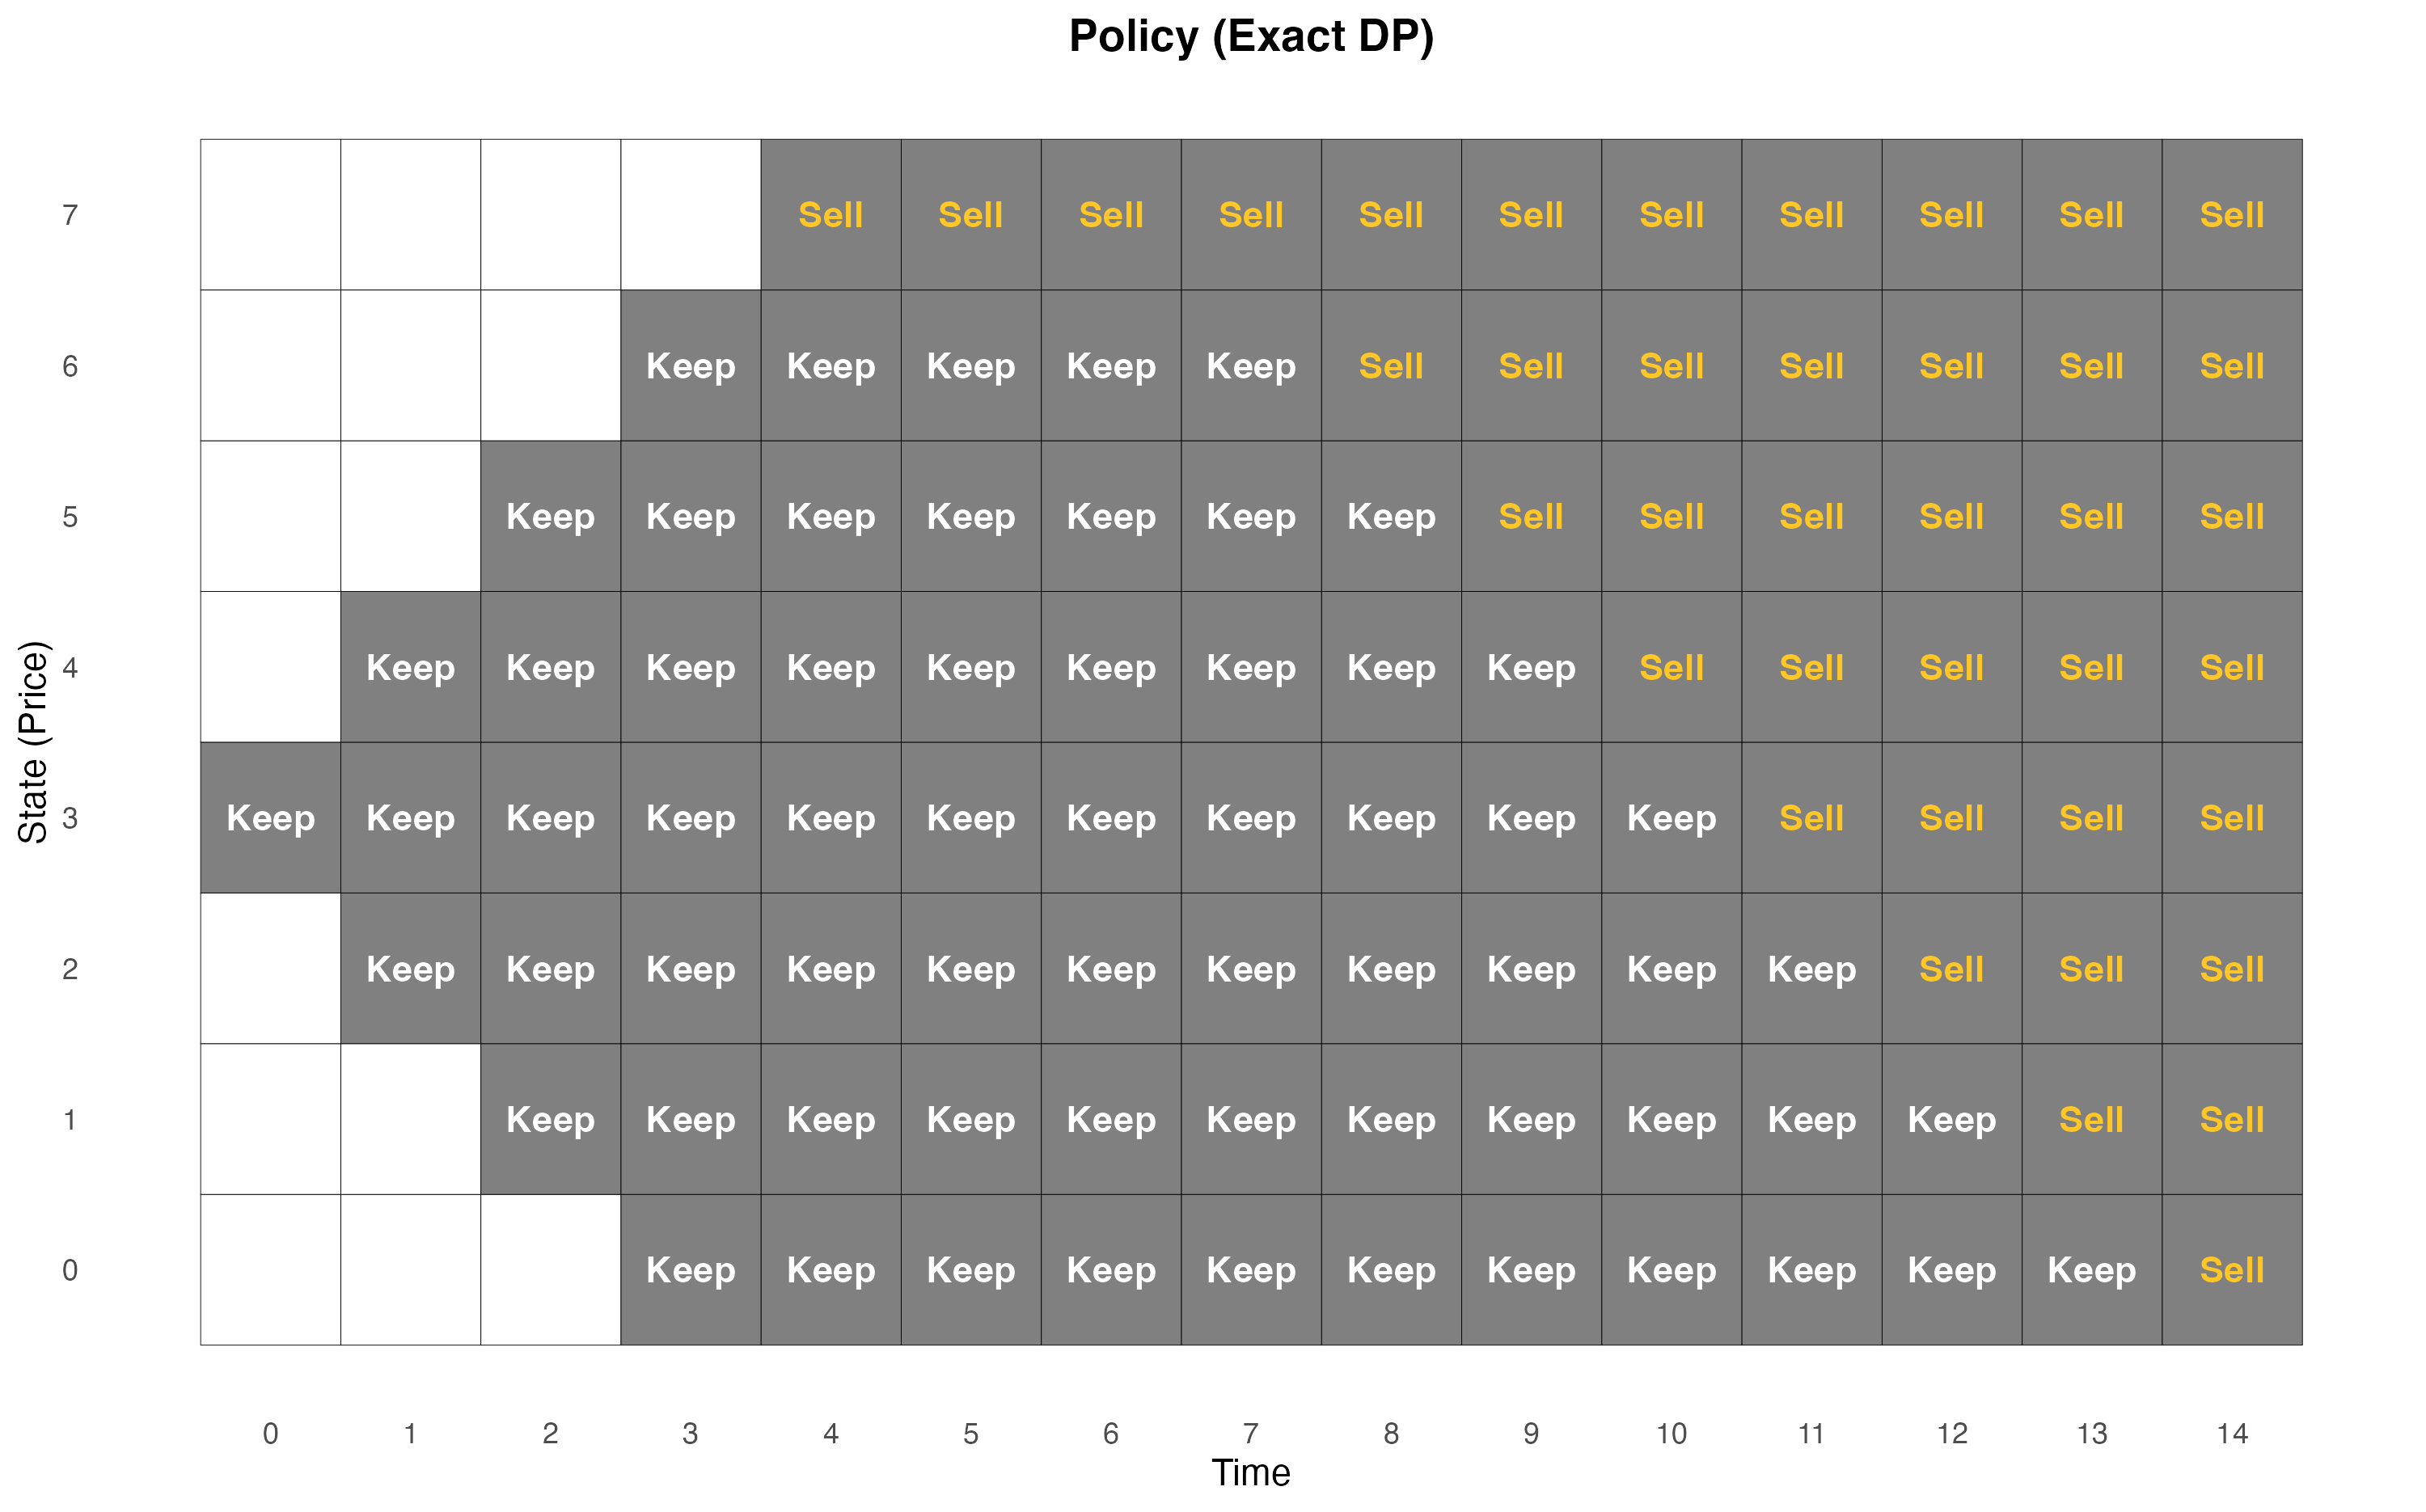
\includegraphics[width=0.9\linewidth, height=6cm]{media/hw2/parta2.png}
    \label{fig:parta2}
    \end{subfigure}
    \caption{Expected rewards and optimal policy at each state and time by exact dynamic programming. The initial expected rewards is 3.233}
    \label{fig:parta}
    \end{figure}

    \item
    The base heuristic specifies a sell condition that is associated with a referencing price $x_0$ and a return rate $\beta$. We generalize the idea with the reward-to-go function in the following way:
    
    Assume the investment starts at time $k$ with state $x_k$, the reward-to-go at time $n$ is denoted as 
    \[
    J^{x_k}_n(x_n), n \in (k, \dots, N),
    \]
    where $x_k$ is the starting/referencing state and $k$ is the starting time.

    The approximated reward-to-go function $\tilde{J}^k_n(x_n)$ is given by
    \[
    \tilde{J}^{x_k}_N(x_N) = x_N
    \]
    and if $k \le n < N$,
    \begin{equation}
    \tilde{J}^k_n(x_n) = 
    \begin{cases}
        \bar x, & x_n = \bar x, \\
        x_n, & x_n > \beta x_k, \\
        \begin{split}
          \max \{x_k, E_{\boldsymbol p}[\tilde{J}^{x_k}_{n+1}(f^*(x_n))] \}, 
        \end{split} & \text{otherwise}.
    \end{cases}
    \end{equation}
    The last condition is compatible with the case when $x_n = 0$.
    We slightly modify the base heuristic to strictly large ($x_k > \beta x_0$) to avoid the case that when $x_0 = 0$, the best option is to sell immediately.
    The base heuristic policy $\tilde \pi$ is determined as,
    \[
    \tilde u_k = \begin{cases}
        1 ~(\text{Sell}) & \text{if } x_k = \tilde{J}_k^{x_0}(x_k), \\
        0 ~(\text{Keep}) & \text{otherwise}.
    \end{cases}
    \]
    The expected reward and policy computed by base heuristic with starting point $x_0$ is shown in Fig. (\ref{fig:partb}).

    \begin{figure}[h]
    \begin{subfigure}{0.5\textwidth}
    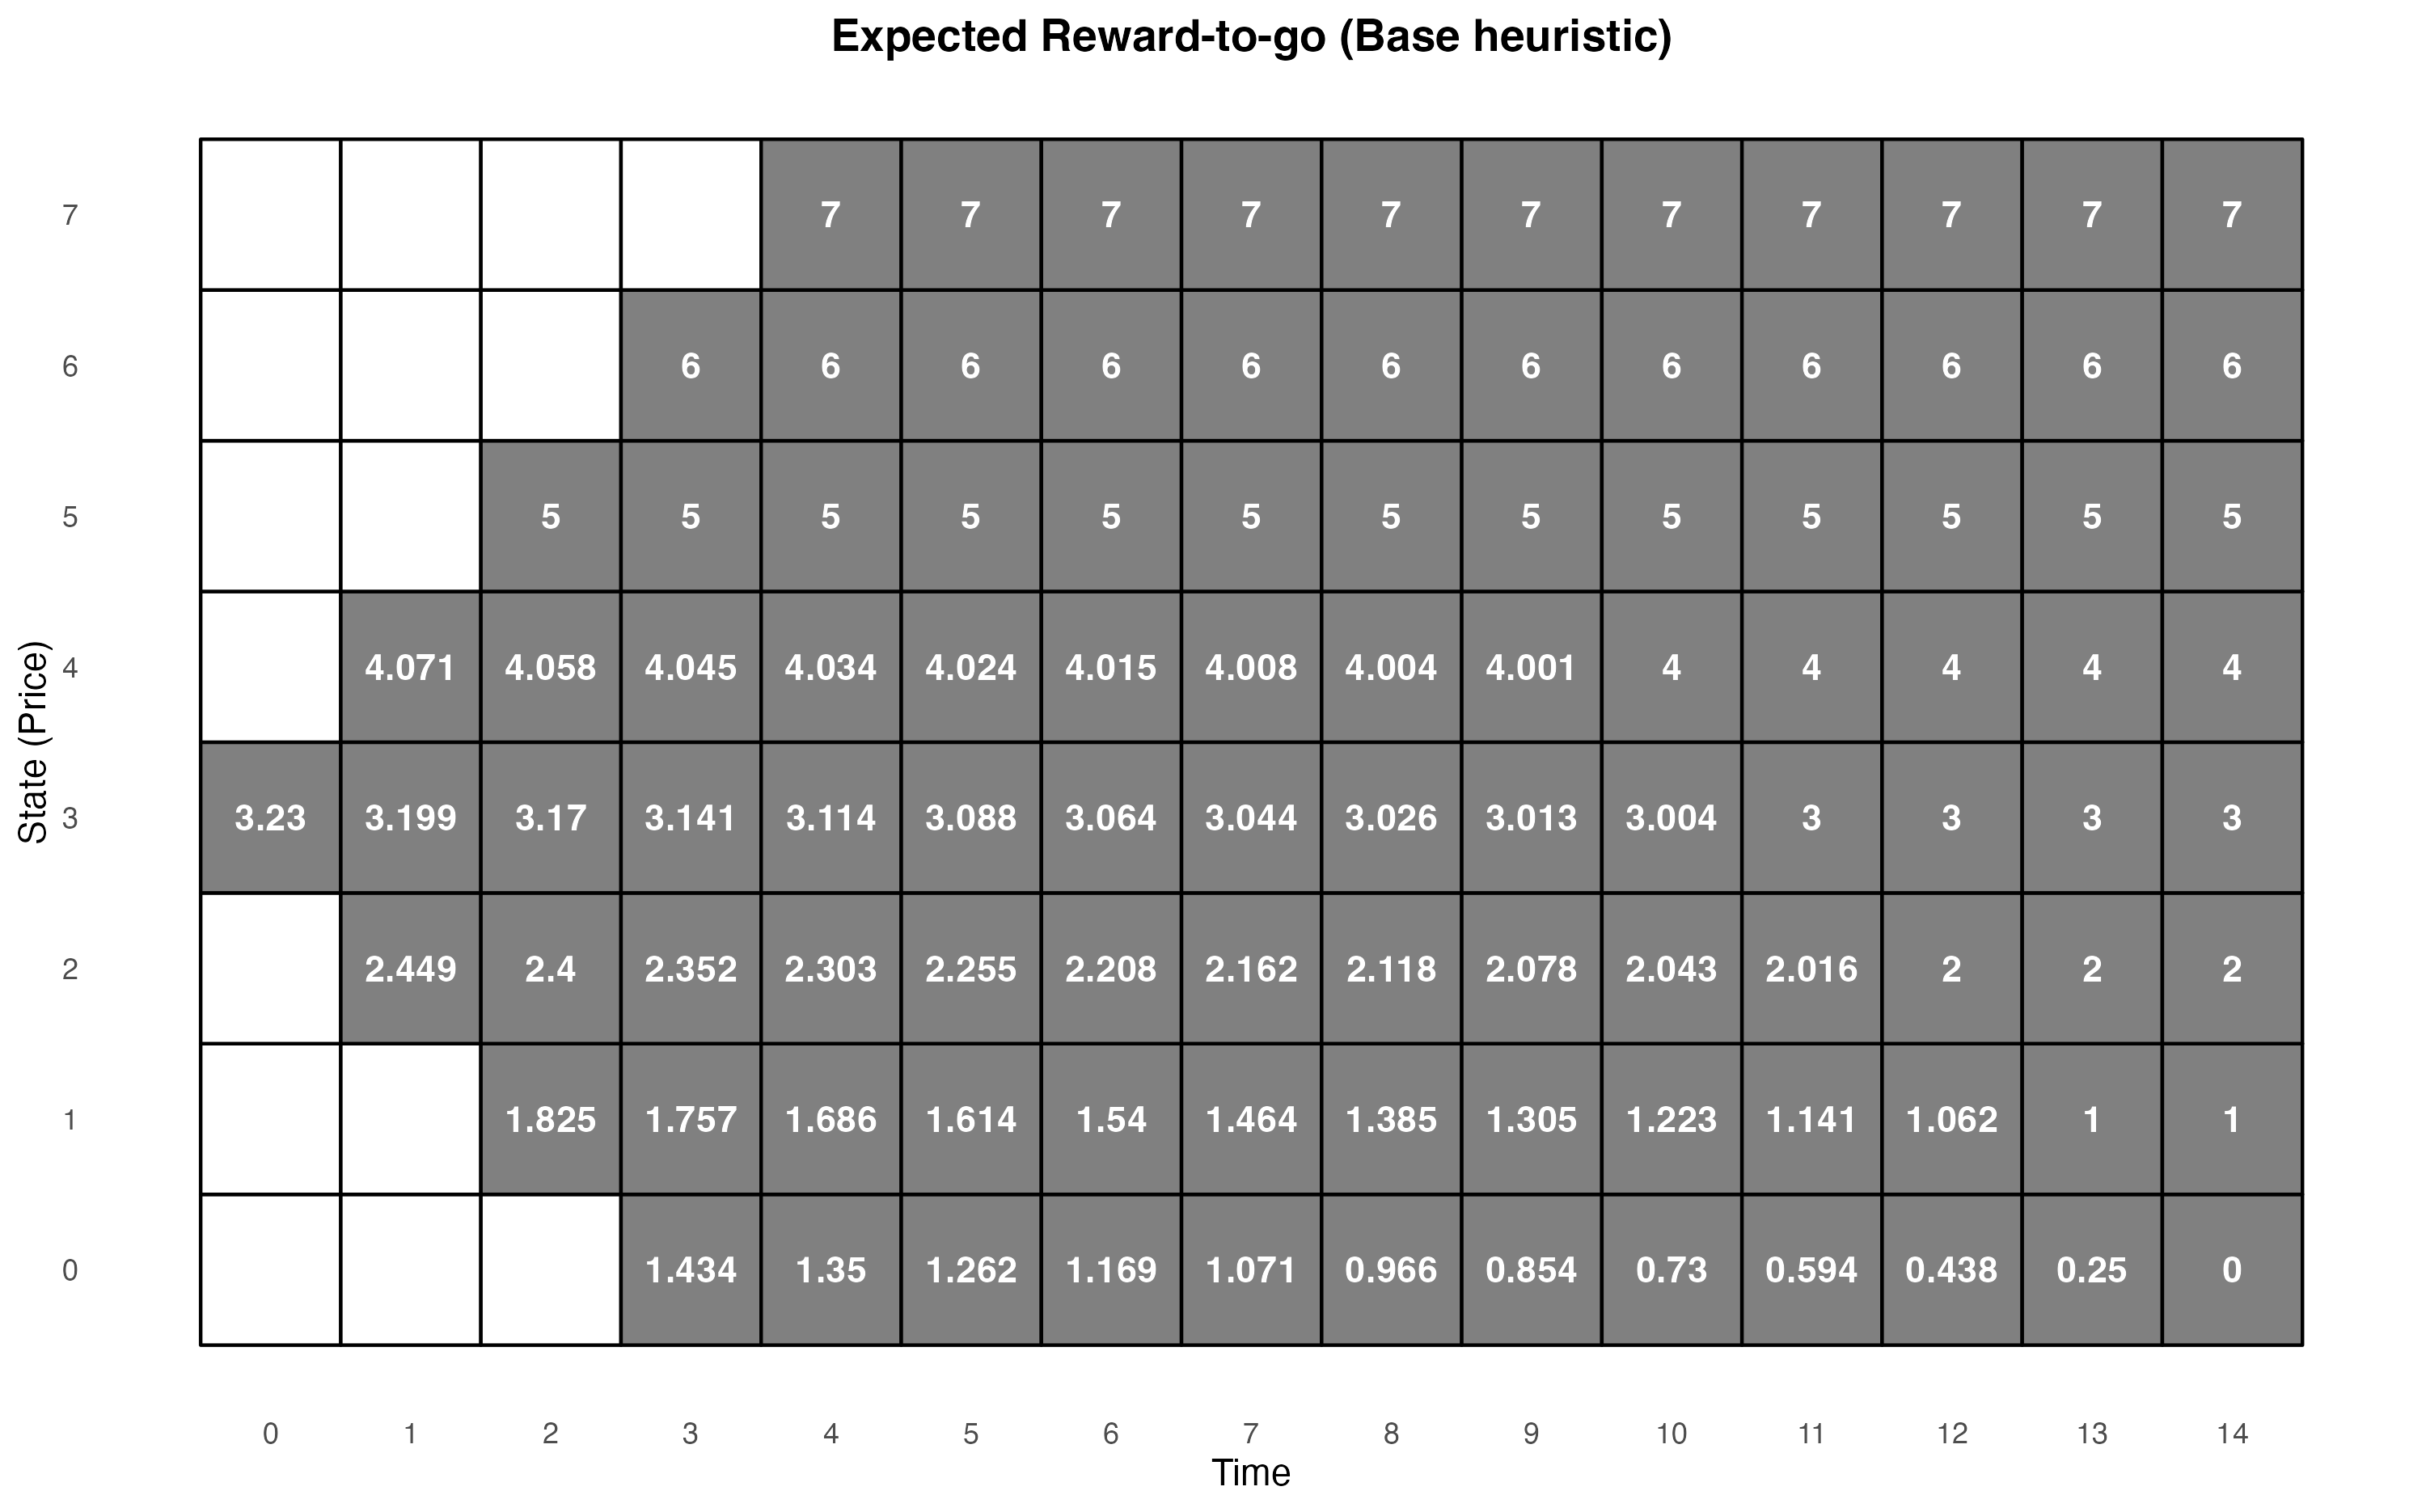
\includegraphics[width=0.9\linewidth, height=6cm]{media/hw2/partb1.png} 
    \label{fig:partb1}
    \end{subfigure}
    \begin{subfigure}{0.5\textwidth}
    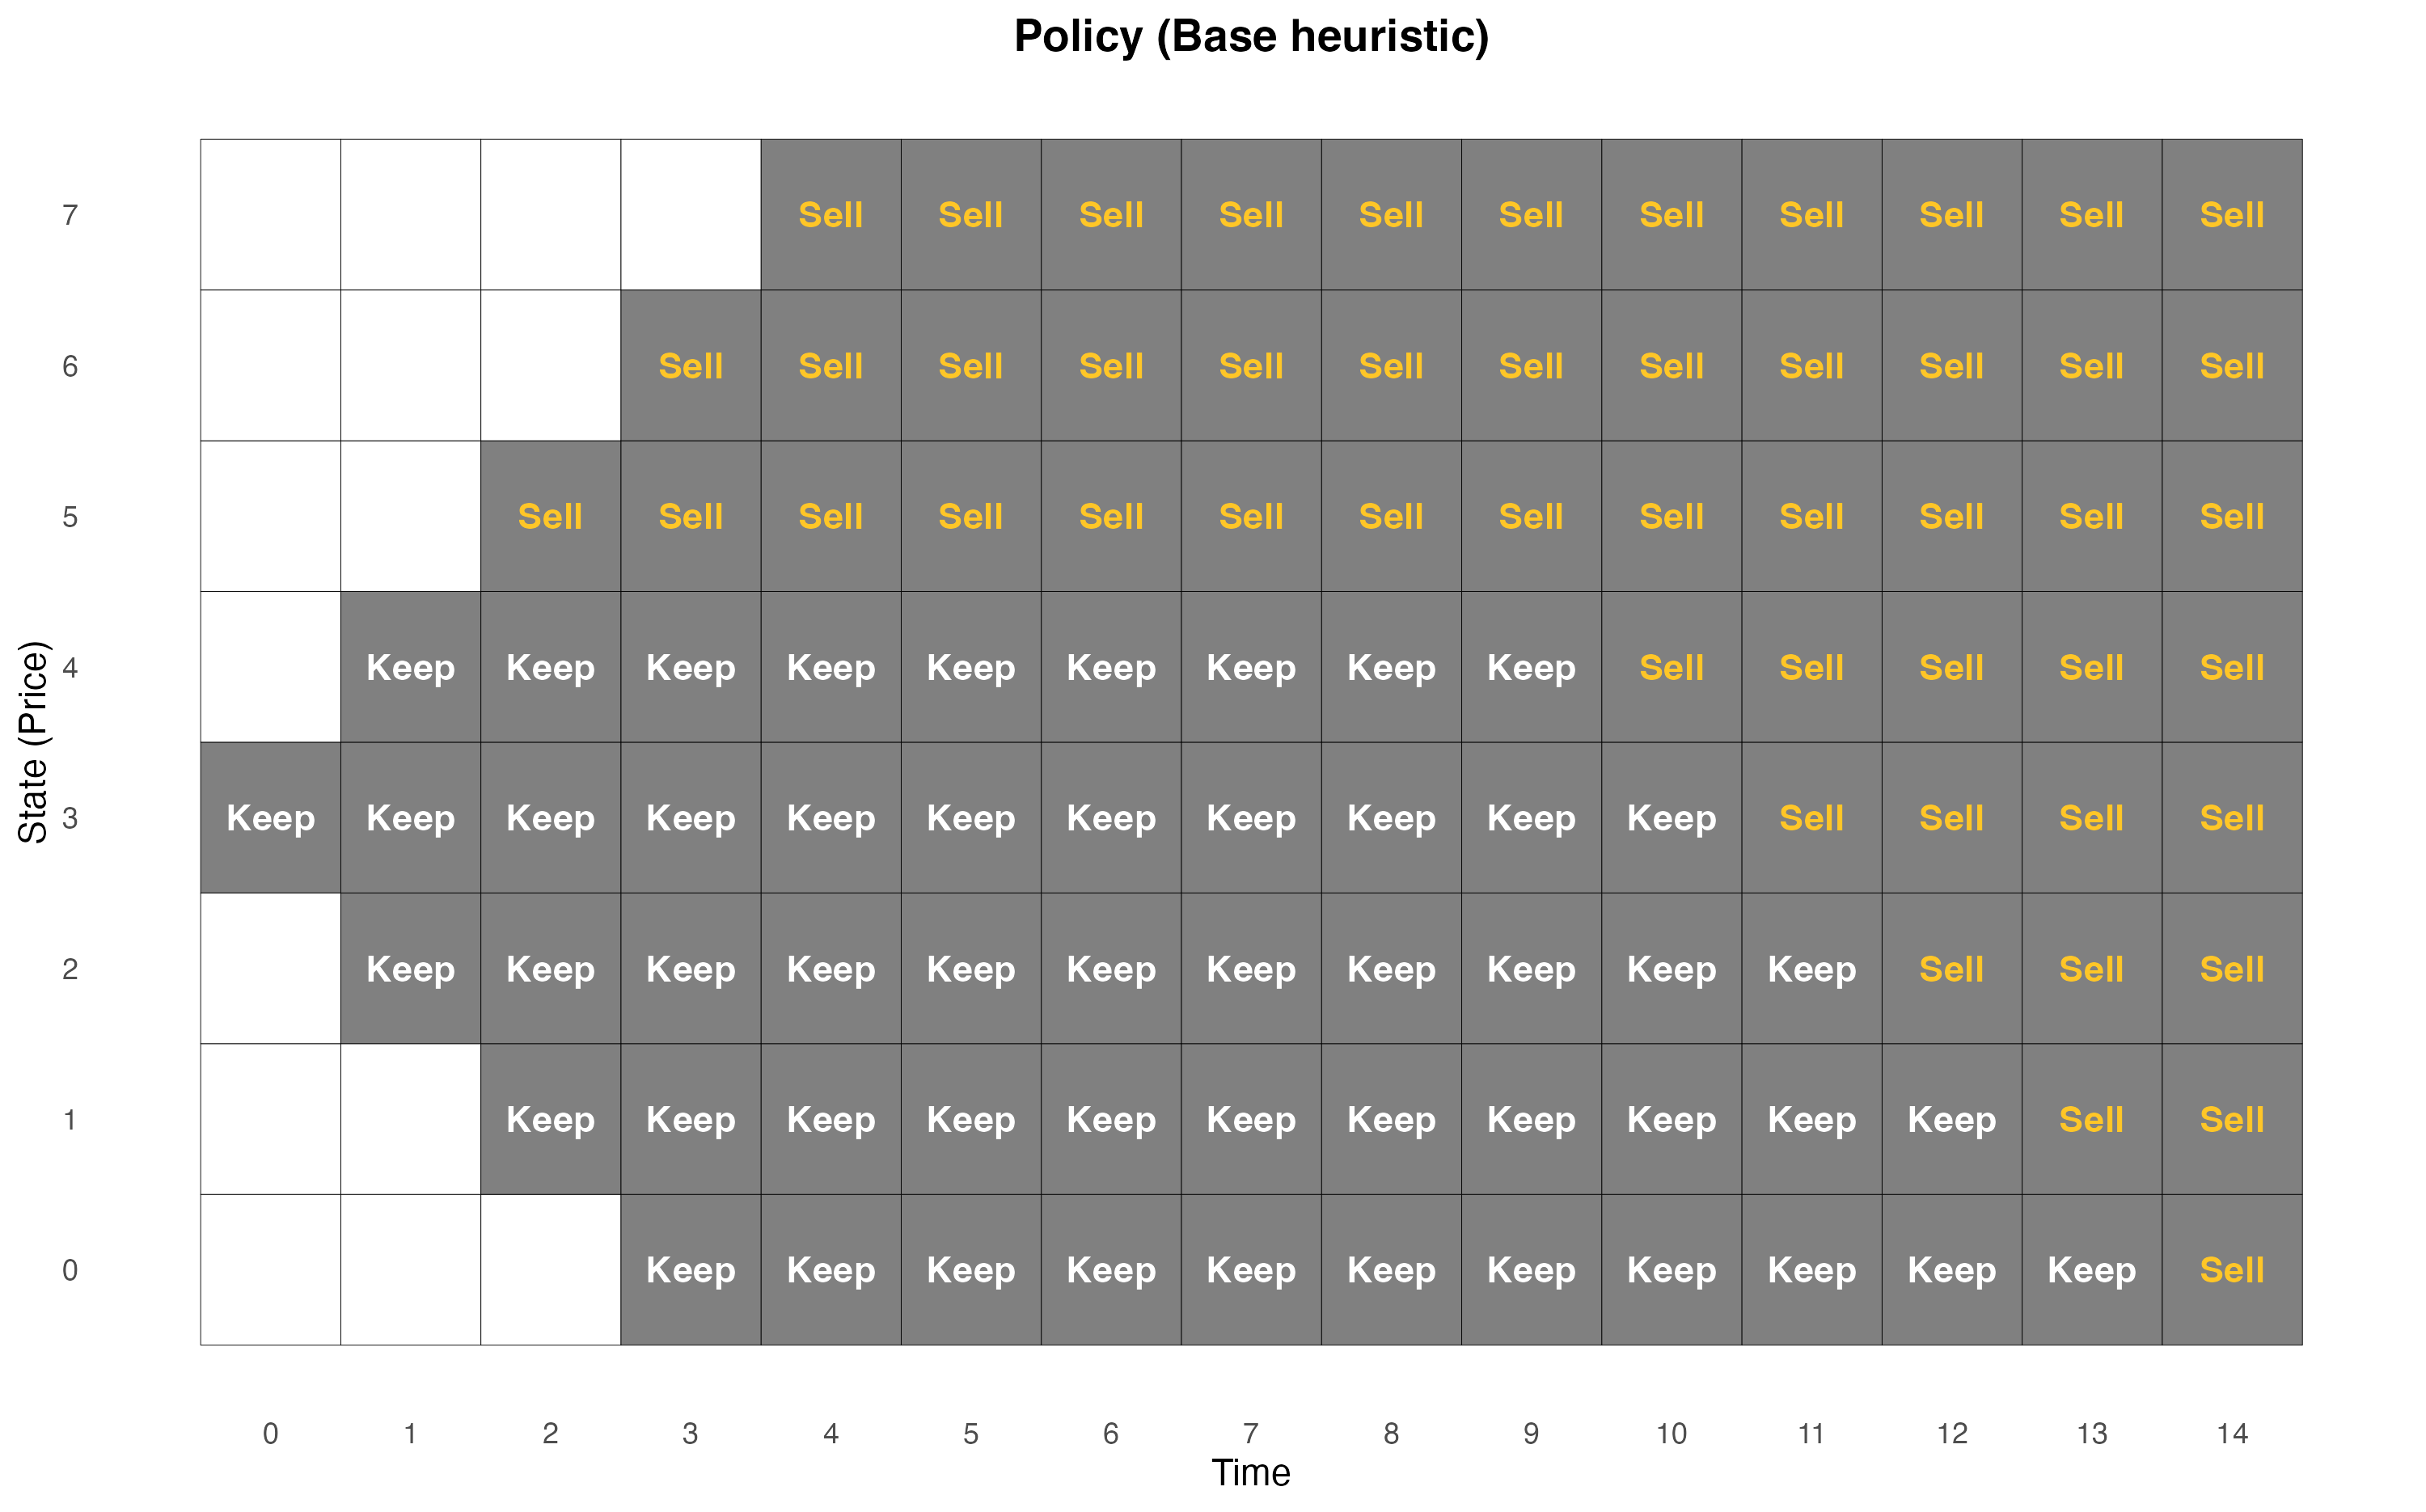
\includegraphics[width=0.9\linewidth, height=6cm]{media/hw2/partb2.png}
    \label{fig:partb2}
    \end{subfigure}
    \caption{Expected rewards and policy by base heuristic ($\beta = 1.4$). The initial expected rewards is 3.23}
    \label{fig:partb}
    \end{figure}
    
    The base heuristic is simple and efficient to implement. We only need to compare current price and the expected reward, which is computed with $(J^{x_k + 1}_{k+1}(x_k+1), J^{x_k }_{k+1}(x_k), J^{x_k - 1}_{k+1}(x_k-1))$.
    However, the reward $\$3.23$ is sub-optimal compared to $\$3.233$ in part(a).
    
    \item
    The one-step rollout policy is an extension to the algorithm in part(b). The base heuristic policy makes the sell decision based on the initial price $x_0$, while the rollout policy considers the feedback at each stage to make the decision. Specifically, the rollout policy $\tilde \pi = \{\tilde u_0, \dots, \tilde u_{N-1}\}$ is determined as
    \[
    \tilde u_k = \begin{cases}
        1~(\text{Sell}) & \text{if } x_k = \tilde{J}_k(x_k), \\
        0~(\text{Keep}) & \text{otherwise},
    \end{cases}
    \]
    where the approximated reward-to-go function $\tilde{J}_k(x_k)$ is given by
    \[
    \tilde{J}_N(x_N) = x_N,
    \]
    if $k = N$. For $k = 1, \dots, N - 1 $, $\tilde{J}_k(x_k)$ is defined as
    \begin{equation}
    \tilde{J}_k(x_k) = 
    \begin{cases}
        \bar x, & x_n = \bar x, \\
        \max \{x_k, E_{\boldsymbol p}[\tilde{J}_{k+1}(f^*(x_k))] \}, & \text{otherwise},
    \end{cases}
    \end{equation}
    where 
    \begin{equation}\label{eq:8}
    E_{\boldsymbol p}[\tilde{J}_{k+1}(f^*(x_k))] = p^+\tilde{J}^{x_k + 1}_{k+1}(x_k + 1) + p^-\tilde{J}^{x_k - 1}_{k+1}(x_k - 1) + (1-p^+-p^-)\tilde{J}^{x_k}_{k+1}(x_k)
    \end{equation}
    It's worth noting that the superscript of $(J^{x_k + 1}_{k+1}(x_k+1), J^{x_k }_{k+1}(x_k), J^{x_k - 1}_{k+1}(x_k-1))$ is different, indicating each item has its own referencing price, i.e. different selling conditions.
    However, unlike the example solution given in the note, my implementation of one-step rollout algorithm gives lower expect rewards for $x_0$.
    As shown in Fig. (\ref{fig:partc}), the expect value is 3.212, compare to 3.23 in part(b) and 3.233 in part(a). The alternative algorithm is to set the referencing state to $x_k$ in Eq. (\ref{eq:8}). However, this will give the same result as in part(b) for $x_0$.

    \begin{figure}[h]
    \begin{subfigure}{0.5\textwidth}
    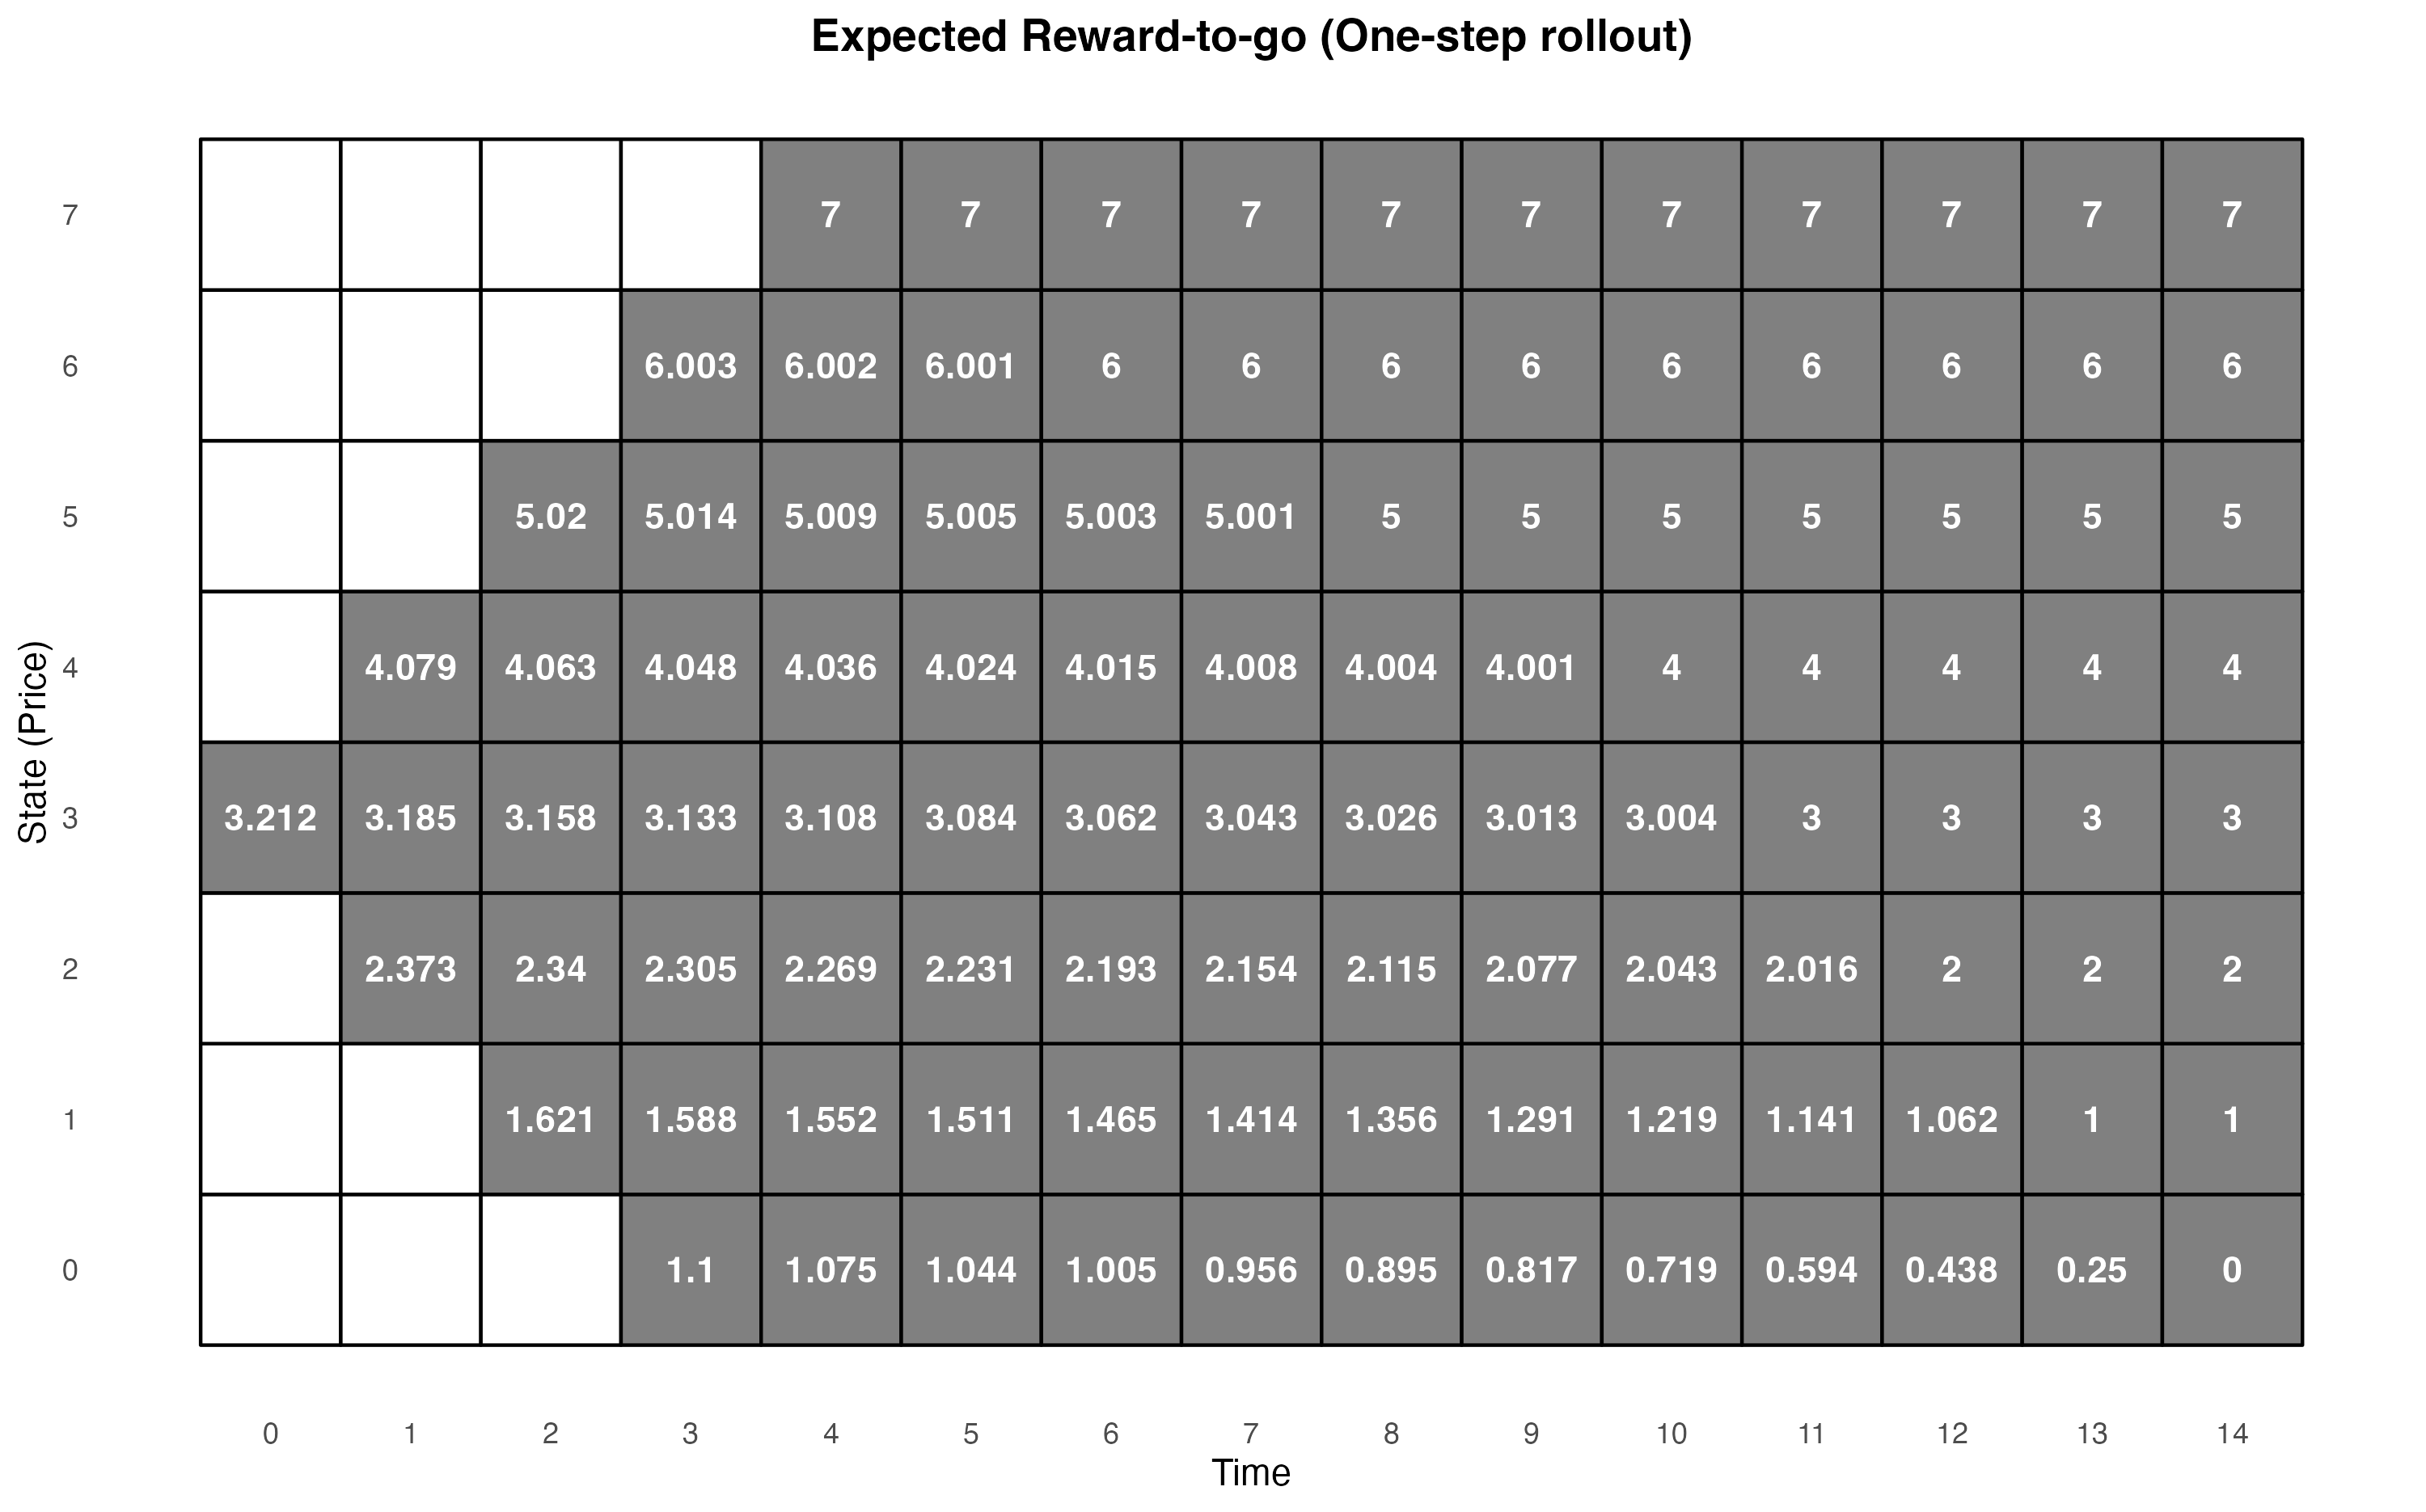
\includegraphics[width=0.9\linewidth, height=6cm]{media/hw2/partc1.png} 
    \label{fig:partc1}
    \end{subfigure}
    \begin{subfigure}{0.5\textwidth}
    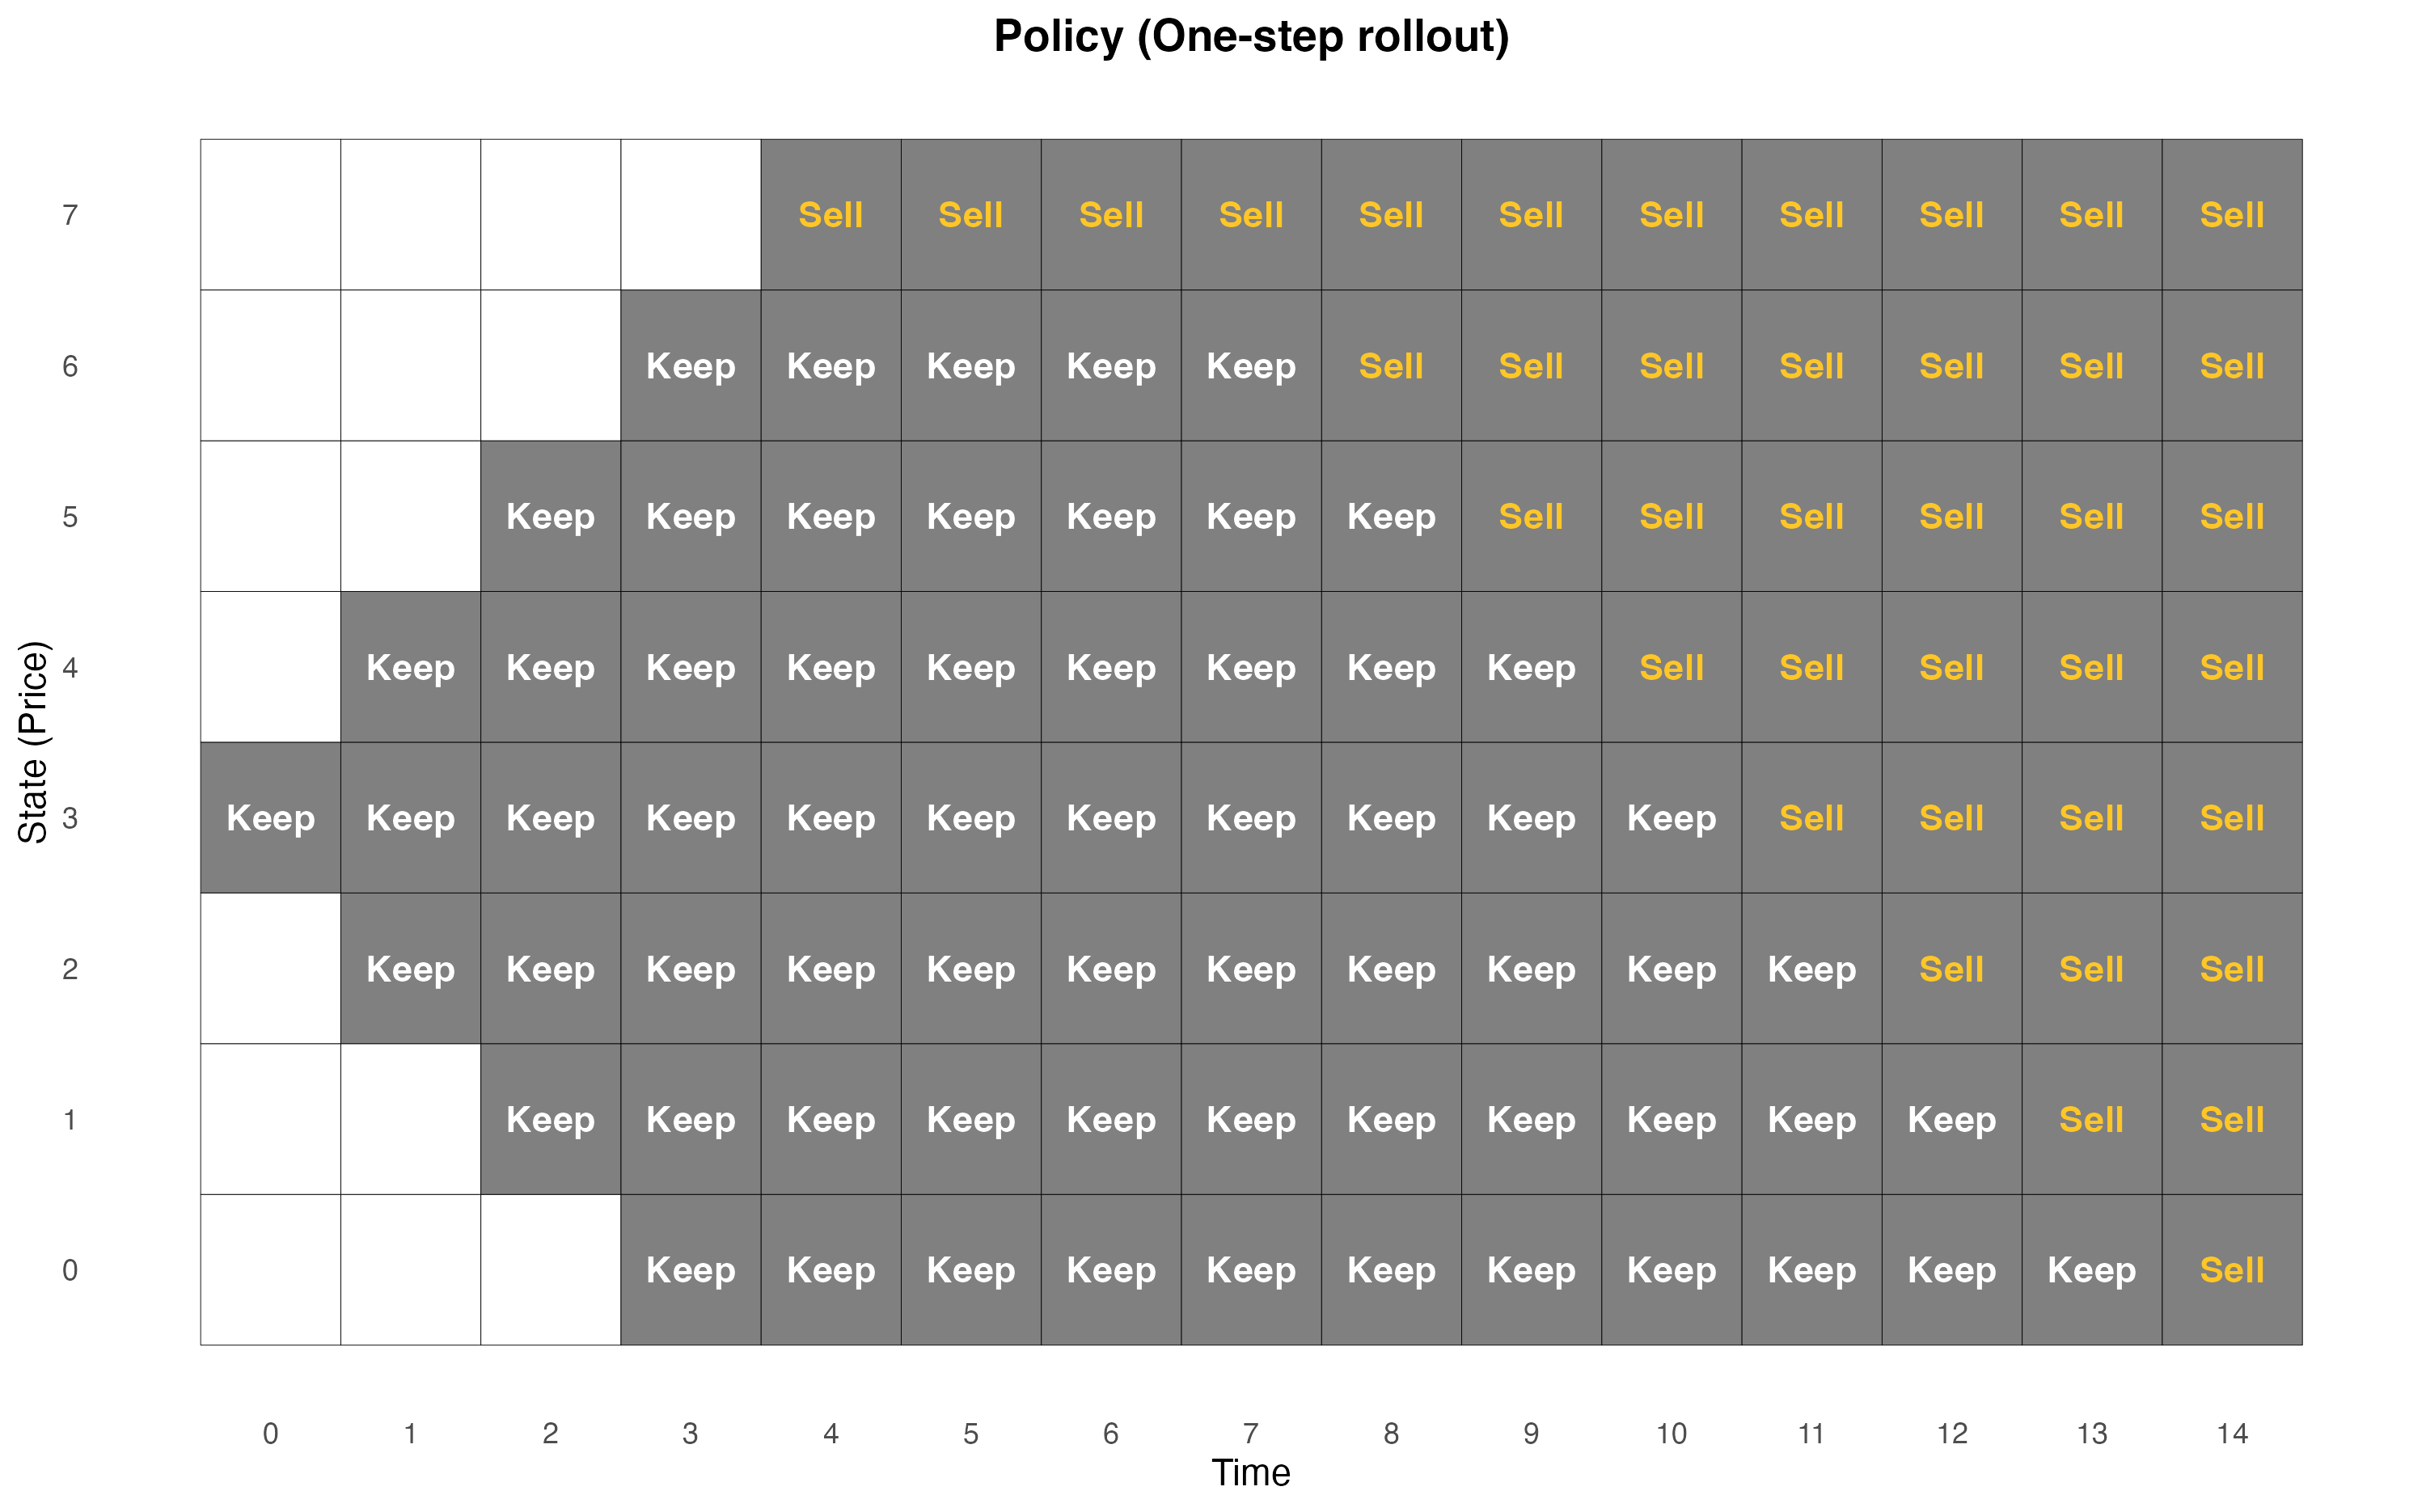
\includegraphics[width=0.9\linewidth, height=6cm]{media/hw2/partc2.png}
    \label{fig:partc2}
    \end{subfigure}
    \caption{Expected rewards and policy by one-step rollout algorithm ($\beta = 1.4$). The initial expected rewards is 3.212}
    \label{fig:partc}
    \end{figure}

    The computation runtime of one-step lookahead is similar to base heuristic as they both compute three reward-to-go functions $(J^{x_k + 1}_{k+1}(x_k+1), J^{x_k }_{k+1}(x_k), J^{x_k - 1}_{k+1}(x_k-1))$. An alternative efficient algorithm is Monte Carlo simulation, which generate multiple possible trajectories from starting state $x_k$, and then averaging the sample rewards to replace the heuristic approximations.

    The Monte Carlo approximation is unstable when the sample is small, and converges to the true value when sample number increases. We tried three sample numbers (500/1,000/10,000) in the code, with values of 3.2015, 3.16625, 3.212382, respectively. The last one is fairly close to the expect reward one-step rollout algorithm, and the computation speed is much faster.
    
    \item
    Two-step lookahead algorithm is very similar to one-step rollout case. The main difference is that this algorithm needs to calculate 5 rewards values using base heuristic.
    \begin{equation}\label{eq:9}
    x_k = \begin{cases}
        x_k + 1 & \begin{cases}
            x_k + 2 & p^+ \cdot p^+ \\
            x_k + 1 & p^+ \cdot (1-p^+ - p^-) \\
            x_k & p^+ \cdot p^-
        \end{cases} \\
        x_k & \begin{cases}
            x_k + 1 & (1-p^+ - p^-) \cdotp^+ \\
            x_k & (1-p^+ - p^-) \cdot (1-p^+ - p^-)\\
            x_k - 1 & (1-p^+ - p^-) \cdot p^-
        \end{cases} \\
        x_k - 1 & \begin{cases}
            x_k & p^- \cdot p^+ \\
            x_k - 1 & p^- \cdot (1-p^+ - p^-) \\
            x_k - 2 & p^- \cdot p^-
        \end{cases}
    \end{cases}
    \end{equation}
    The 2-step lookahead policy and reward function is similar to the definitions in part(c) (Eq. (\ref{eq:8})), except the expected reward is based on $\tilde{J}_{k+2}$ instead of $\tilde{J}_{k+1}$ and the disturbance distribution $\boldsymbol p$ is based on Eq. (\ref{eq:9}).
    
    Like in part(c), the two-step lookahead algorithm gives unintended lower expect rewards (3.007).
    \begin{figure}[h]
    \begin{subfigure}{0.5\textwidth}
    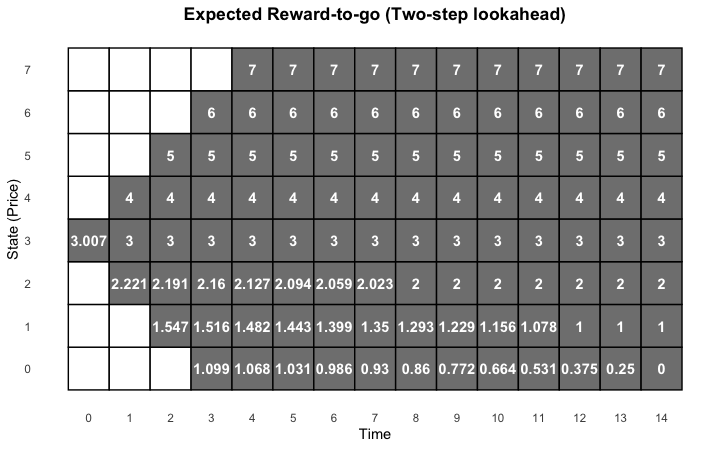
\includegraphics[width=0.9\linewidth, height=6cm]{media/hw2/partd1.png} 
    \label{fig:partd1}
    \end{subfigure}
    \begin{subfigure}{0.5\textwidth}
    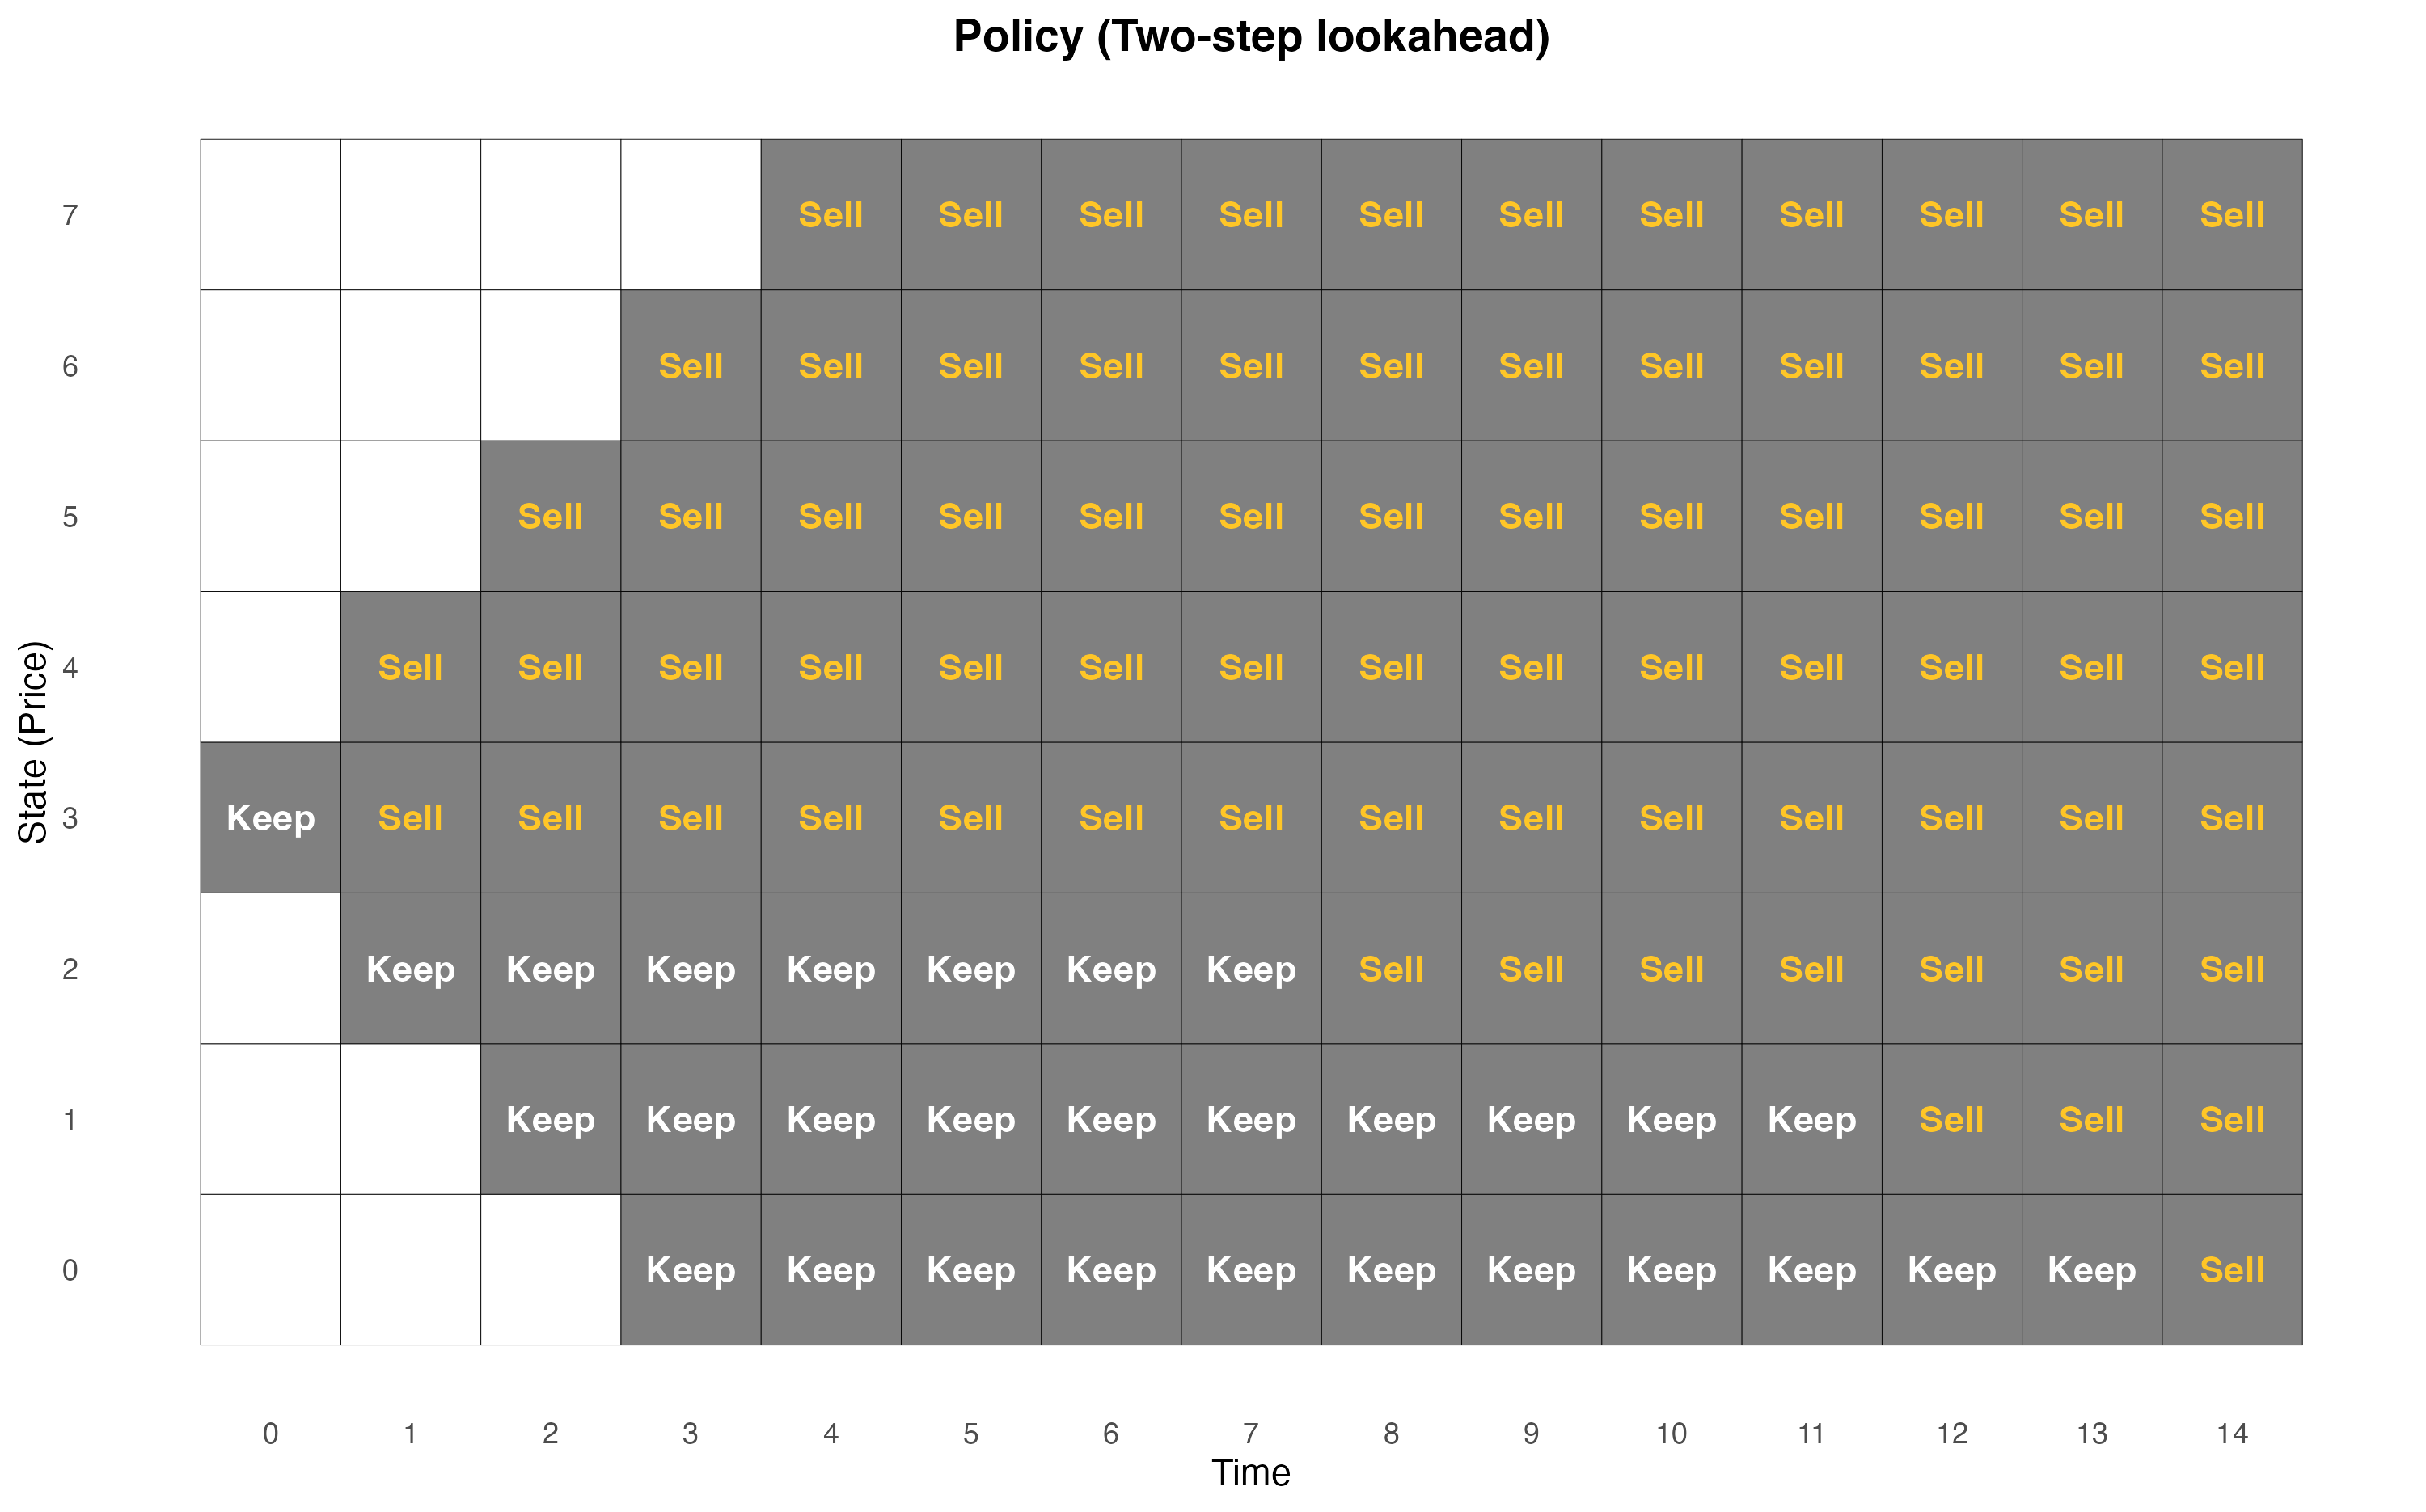
\includegraphics[width=0.9\linewidth, height=6cm]{media/hw2/partd2.png}
    \label{fig:partd2}
    \end{subfigure}
    \caption{Expected rewards and policy by two-step lookahead algorithm ($\beta = 1.4$). The initial expected rewards is 3.007}
    \label{fig:partd}
    \end{figure}
\end{enumerate}

\newpage
\section*{Appendix}
\subsection*{Code}

\lstinputlisting[language=R]{code/hw2.R}

\end{document}